\documentclass[a4paper,12pt]{article}
\usepackage{geometry}
\geometry{left=2.5cm,right=2.5cm,top=2.5cm,bottom=2.5cm}
\renewcommand{\textfraction}{0.15}
\renewcommand{\topfraction}{0.85}
\renewcommand{\bottomfraction}{0.65}
\renewcommand{\floatpagefraction}{0.60}
\usepackage{amsmath}
\usepackage{amsfonts}
\usepackage{mathrsfs}
\usepackage{amsthm}
\usepackage{amssymb}
\usepackage{extarrows}
\usepackage{bm}
\usepackage{graphicx}
\usepackage[section]{placeins}
\usepackage{flafter}
\usepackage{array}
\usepackage{caption}
\usepackage{subcaption}
\usepackage{color}
\usepackage{multirow}
\usepackage{listings}

\DeclareMathOperator*{\argmaxdown}{arg\,max}
\DeclareMathOperator*{\argmindown}{arg\,min}
\DeclareMathOperator{\argmax}{arg\,max}
\DeclareMathOperator{\argmin}{arg\,min}



\title{Solutions of A Probabilit Path}
\author{Chao Cheng
  \\
  Github ID: fenguoerbian
  \\
  Mail: 413557584@qq.com}
\date{\today}



\begin{document}
\maketitle

\section{Solutions to Chapter 1: Sets and Events}
\label{sec:solutions-chapter-1}

\newcounter{Lcount}
\setcounter{Lcount}{0}
\begin{list}{1.9.\arabic{Lcount}}{\usecounter{Lcount}}
\item \label{ex.1.9.1}
  $\forall B \in \aleph$, since $\mathcal{C}\subset B$, we have $\{0\}\in B$, therefore $\Omega\setminus \{0\}=\{1\}\in B$. Also $\emptyset\in B$ and $\Omega\in B$. Therefore $\{\emptyset,\{0\}, \{1\}, \Omega\}\subset B$. Note that $\mathcal{P}\left(\Omega\right) = \{\emptyset,\{0\}, \{1\}, \Omega\}$. This means
  \[
    \aleph = \{\mathcal{P}\left(\Omega\right)\}
  \]
\item \label{ex.1.9.2}Like in 1.9.\ref{ex.1.9.1}, we can conclude that
  \[
    \forall B \in \aleph \quad \Rightarrow \left\{\emptyset, \{0\}, \{1,2\}, \Omega\right\} \subset B
  \]
  Also note that $\left\{\emptyset, \{0\}, \{1,2\}, \Omega\right\}$ is a $\sigma$-field itself which means
  \[
    \sigma\left(\mathcal{C}\right) = \left\{\emptyset, \{0\}, \{1,2\}, \Omega\right\}
  \]
  Those subsets of $\Omega$ which are not included in $\sigma(\mathcal{C})$ are
  \[
    \{1\},\quad \{2\},\quad \{0,1\},\quad \{0,2\}
  \]
  and it's easy to check that they are all included in $B$ if any one of them is inclued. So to sum up, we have
  \[
    \aleph = \left\{\sigma(\mathcal{C}), \mathcal{P}\left(\Omega\right)\right\}
  \]
\item \label{ex.1.9.3} Firstly
  \[
    \begin{aligned}
      \underset{n\to\infty}{\mathrm{lim\,sup}} A_n\cup B_n
      &= \left\{x\middle| \sum\limits_{n=1}^\infty 1_{A_n\cup B_n}\left(x\right)=\infty\right\}    \\
      &= \left\{x\middle| \sum\limits_{n=1}^\infty 1_{A_n}\left(x\right)=\infty\quad \mathrm{or}\quad
         \sum\limits_{n=1}^\infty 1_{B_n}\left(x\right)=\infty\right\}    \\
      &= \left\{x\middle| \sum\limits_{n=1}^\infty 1_{A_n}\left(x\right)=\infty \right\} \cup
         \left\{x\middle| \sum\limits_{n=1}^\infty 1_{B_n}\left(x\right)=\infty\right\}    \\
      &= \underset{n\to\infty}{\mathrm{lim\,sup}} A_n \cup \underset{n\to\infty}{\mathrm{lim\,sup}} B_n
    \end{aligned}
  \]
  Secondly, the statement
  \[
    A_n\cup B_n \to A\cup B,\quad A_n\cap B_n \to A \cap B
  \]
  is true if $A_n\to A$ and $B_n \to B$. Because we have
  \[
    \begin{aligned}
      & \underset{n\to\infty}{\mathrm{lim\,sup}} A_n
      = \underset{n\to\infty}{\mathrm{lim\,inf}} A_n
      = \underset{n\to\infty}{\mathrm{lim}} A_n = A    \\
      & \underset{n\to\infty}{\mathrm{lim\,sup}} B_n
      = \underset{n\to\infty}{\mathrm{lim\,inf}} B_n
      = \underset{n\to\infty}{\mathrm{lim}} B_n = B
    \end{aligned}
  \]
  Using the result of the first problem we can deduce that
  \[
    \underset{n\to\infty}{\mathrm{lim\,sup}} A_n\cup B_n =
    \underset{n\to\infty}{\mathrm{lim\,sup}} A_n \cup \underset{n\to\infty}{\mathrm{lim\,sup}} B_n
    = A \cup B
  \]
  We now have to show that
  \[
    \underset{n\to\infty}{\mathrm{lim\,inf}} A_n \cup B_n =
    \underset{n\to\infty}{\mathrm{lim\,inf}} A_n \cup \underset{n\to\infty}{\mathrm{lim\,inf}} B_n
    = A \cup B
  \]
  Or equally
  \[
    \underset{n\to\infty}{\mathrm{lim\,sup}} A_n \cup B_n
    \subset
    \underset{n\to\infty}{\mathrm{lim\,inf}} A_n \cup B_n
  \]
  \[
    \begin{aligned}
      & x \in \underset{n\to\infty}{\mathrm{lim\,sup}} A_n \cup B_n
      \iff x \in A \cup B
      \iff \underset{n\to\infty}{\mathrm{lim\,inf}} A_n \cup \underset{n\to\infty}{\mathrm{lim\,inf}} B_n\\
      \iff&
      \left\{x \notin A_n\text{, finitely}\right\} \text{ or } \left\{x \notin B_n\text{, finitely}\right\}    \\
      \implies& \left\{ x \notin A_n \cup B_n \text{, finitely}\right\}
      \iff x \in \underset{n\to\infty}{\mathrm{lim\,inf}} A_n \cup B_n
    \end{aligned}
  \]
  This means $\forall x\in \underset{n\to\infty}{\mathrm{lim\,sup}} A_n \cup B_n$, we have that $x\in\underset{n\to\infty}{\mathrm{lim\,inf}} A_n \cup B_n$, therefore
  \[
    \underset{n\to\infty}{\mathrm{lim\,sup}} A_n \cup B_n
    \subset
    \underset{n\to\infty}{\mathrm{lim\,inf}} A_n \cup B_n
  \]
  which means
  \[
    A_n \cup B_n \to A \cup B
  \]
  and
  \[
    A_n \cap B_n = \left(A_n^c \cup B_n^c\right)^c \to \left(A^c \cup B_c\right)^c = A \cap B
  \]
\item \label{ex.1.9.4}
  \[
    \begin{aligned}
      \underset{n\to\infty}{\mathrm{lim\,inf}} A_n &= \bigcup\limits_{n=1}^\infty \bigcap\limits_{k=n}^\infty A_k    \\
      &= \bigcup\limits_{n=1}^\infty \bigcap\limits_{k=n}^\infty \left\{
        \frac{m}{k}:m\in\mathbb{N}
      \right\}    \\
      &= \bigcup\limits_{n=1}^\infty \mathbb{N} = \mathbb{N}
    \end{aligned}
  \]
  \[
    \begin{aligned}
      \underset{n\to\infty}{\mathrm{lim\,sup}} A_n &= \bigcap\limits_{n=1}^\infty \bigcup\limits_{k=n}^\infty A_k    \\
      &= \bigcap\limits_{n=1}^\infty \bigcup\limits_{k=n}^\infty \left\{
        \frac{m}{k}:m\in\mathbb{N}
      \right\}    \\
      &= \bigcap\limits_{n=1}^\infty\mathbb{Q^+} = \mathbb{Q^+}
    \end{aligned}
  \]
  
\item
  \[
    \begin{aligned}
      & \left\{\omega:f_n\left(\omega\right)\nrightarrow f\left(\omega\right)\right\}    \\
      \iff & \left\{\omega: \exists\;\epsilon > 0,\;\mathrm{s.t.}\;\forall N,\;\exists\;n>N,\;\mathrm{s.t.}\;
        \left|f_n\left(\omega\right) - f\left(\omega\right)\right|>\epsilon
      \right\}    \\
      \iff & \bigcup\limits_{k=1}^\infty\bigcap\limits_{N=1}^\infty\bigcup\limits_{n=N}^\infty
      \left\{
        \omega:\left|f_n\left(\omega\right) - f\left(\omega\right)\right| > \frac{1}{k}
      \right\}
    \end{aligned}
  \]
  
\item
  Use Lemma 1.3.1, we can conclude that
  \[
    \underset{n\to\infty}{\mathrm{lim\,sup}}\,A_n = \underset{n\to\infty}{\mathrm{lim\,inf}}\,A_n
    = \left(0,\;1\right]
  \]
\item 
  \begin{enumerate}
  \item Since $\theta = 1/8 $, the period is $T=8$. And there are actually 2 distinguished squares. Hence $ \underset{n\to\infty}{\mathrm{limsup}}\;I_n$ is the star area covered by at least one squate and $ \underset{n\to\infty}{\mathrm{liminf}}\;I_n$ is the area covered by both squares. Refer to Figure~\ref{fig:1.9.7.a} as illustration.
    \begin{figure}[htbp]
      \centering
      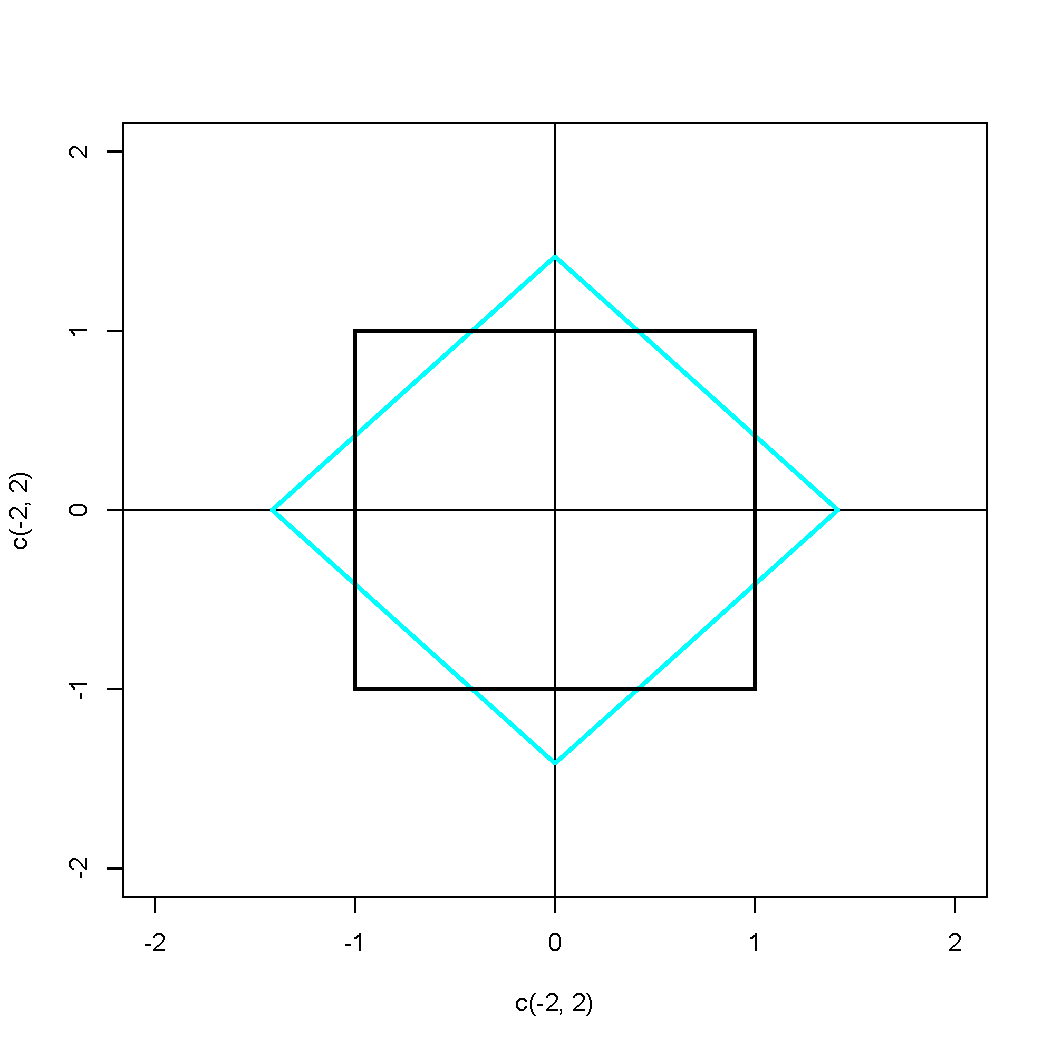
\includegraphics[width=0.5\textwidth]{./Figures/1_9_7_a.pdf}
      \caption{(a)}
      \label{fig:1.9.7.a}
    \end{figure}

  \item If $\theta$ is rational, then it can be written in the form $\theta = \frac{m}{n}$ where both $m$ and $n$ are integers, which means there is a period in $I_n$. Hence like before, $ \underset{n\to\infty}{\mathrm{limsup}}\;I_n$ is the star area covered by at least one squate and $ \underset{n\to\infty}{\mathrm{liminf}}\;I_n$ is the area covered by all squares. Refer to Figure~\ref{fig:1.9.7.b} as illustration.
    \begin{figure}[htbp]
      \centering
      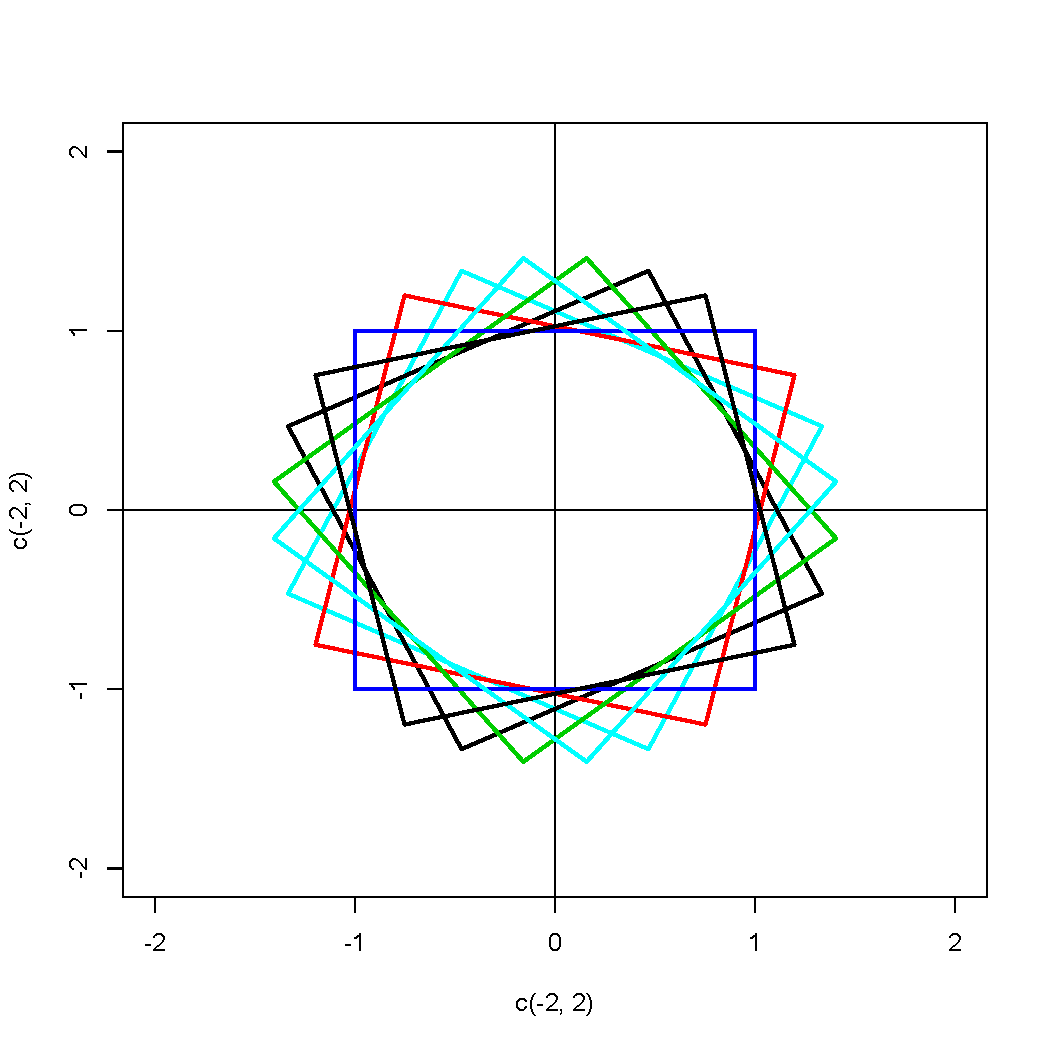
\includegraphics[width=0.5\textwidth]{./Figures/1_9_7_b.pdf}
      \caption{(b) $\theta = \frac{1}{7}$}
      \label{fig:1.9.7.b}
    \end{figure}
    
  \item If $\theta$ is irrational. These squares becomes dense and $ \underset{n\to\infty}{\mathrm{limsup}}\;I_n$ is the round area with radius $r_{\mathrm{sup}}= \sqrt{2}$ and $ \underset{n\to\infty}{\mathrm{liminf}}\;I_n$ is the round area with radius $r_{\mathrm{inf}} = 1$. Refer to Figure~ as illustration.
    \begin{figure}[htbp]
      \centering
      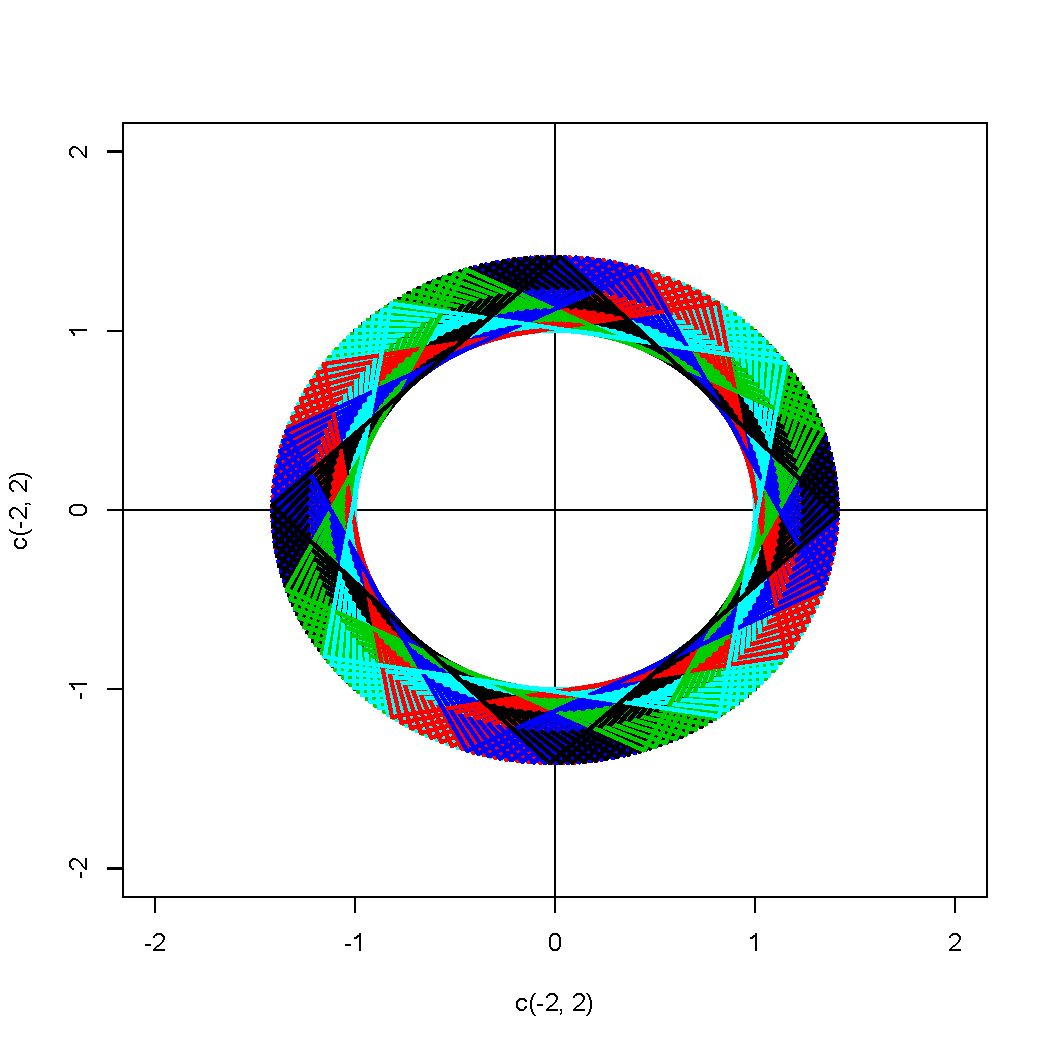
\includegraphics[width=0.5\textwidth]{./Figures/1_9_7_c.pdf}
      \caption{(c) $\theta = e^{1/2}$}
      \label{fig:1.9.7.c}
    \end{figure}
  \item Codes for drawing these figures are provided below:
    \lstinputlisting[language=R]{./Codes/ex_1_9_7_plot.r}
  \end{enumerate}

  
\item
  \[
    \mathrm{limsup}A_n = \bigcap\limits_{n=1}^\infty\bigcup\limits_{k=n}^\infty A_k = B \cup C
  \]
  and
  \[
    \mathrm{liminf}A_n = \bigcup\limits_{n=1}^\infty\bigcap\limits_{k=n}^\infty A_k = B \cap C
  \]

  
\item
  \[
    \begin{aligned}
      A \bigtriangleup B &= \left(A \setminus B\right) \cup \left(B \setminus A\right)    \\
      & = \left(A \cap B^c \right) \cup \left(B \cap A^c \right)    \\
      & = \left(B^c \cap \left(A^c\right)^c \right) \cup \left(A^c \cap \left(B^c\right)^c \right)    \\
      & = \left(B^c \setminus A^c \right) \cup \left(A^c \setminus B^c \right)    \\
      & = A^c \bigtriangleup B^c
    \end{aligned}
  \]

  
\item $\Longrightarrow$:
  \par
  Since $A_n \rightarrow A$, we have
  \[
    \underset{n\to\infty}{\mathrm{lim\,inf}}A_n = \underset{n\to\infty}{\mathrm{lim\,sup}}A_n = A
  \]
  If $w \in A\quad\implies\quad w \in \underset{n\to\infty}{\mathrm{lim\,inf}A_n}$, then
  \[
    \begin{aligned}
      & \exists\;n_0,\quad\text{s.t. }\forall\; n \geq n_0,\quad w \in A_n    \\
      \implies & \forall\; n \geq n_0, 1_{A_n}(w) = 1    \\
      \implies & \underset{n\to\infty}{\mathrm{lim}}\,1_{A_n}\left(w\right) = 1 = 1_{A}\left(w\right)
    \end{aligned}
  \]
  And if $ w \in A^c$, then $w \in \left(\underset{n\to\infty}{\mathrm{lim\,sup}}\,A_n\right)^c = \underset{n\to\infty}{\mathrm{lim\,inf}}\,A_n^c$, which means
  \[
    \begin{aligned}
      & \exists\;n_0,\quad\text{s.t. }\forall\; n \geq n_0,\quad w \in A_n^c    \\
      \implies & \forall\; n \geq n_0, 1_{A_n}(w) = 0    \\
      \implies & \underset{n\to\infty}{\mathrm{lim}}\,1_{A_n}\left(w\right) = 0 = 1_{A}\left(w\right)
    \end{aligned}
  \]
  Hence $A_n\rightarrow A \implies 1_{A_n}\rightarrow 1_{A}$.
  \par
  $\Longleftarrow$:
  If $1_A(w) = 1$, then $\underset{n\to\infty}{\mathrm{lim}}1_{A_n}\left(w\right) = 1$, which means
  \[
    \begin{aligned}
      &\exists\; n_0,\quad\text{s.t. }\forall\; n \geq n_0,\quad 1_{A_n}\left(w\right) = 1    \\
      \implies & \forall\; n \geq n_0,\quad w \in A_n    \\
      \implies & w \in \underset{n\to\infty}{\mathrm{lim\,inf}}A_n    \\
      \implies & A \subset \underset{n\to\infty}{\mathrm{lim\,inf}}A_n
    \end{aligned}
  \]
  If $1_A(w) = 0$, then $\underset{n\to\infty}{\mathrm{lim}}1_{A_n}\left(w\right) = 0$, which means
  \[
    \begin{aligned}
      &\exists\; n_0,\quad\text{s.t. }\forall\; n \geq n_0,\quad 1_{A_n}\left(w\right) = 0    \\
      \implies & \forall\; n \geq n_0,\quad w \in A_n^c    \\
      \implies & w \in \underset{n\to\infty}{\mathrm{lim\,inf}}A_n^c = \left(\underset{n\to\infty}{\mathrm{lim\,sup}}A_n\right)^c    \\
      \implies & A^c \subset \left(\underset{n\to\infty}{\mathrm{lim\,sup}}A_n\right)^c    \\
      \implies & A \subset \underset{n\to\infty}{\mathrm{lim\,sup}}A_n
    \end{aligned}
  \]
  Therefore $\underset{n\to\infty}{\mathrm{lim\,sup}}A_n \subset \underset{n\to\infty}{\mathrm{lim\,inf}}A_n$, which means
  \[
    \underset{n\to\infty}{\mathrm{lim\,inf}}A_n = \underset{n\to\infty}{\mathrm{lim\,sup}}A_n = A
  \]
  Therefore $1_{A_n}\rightarrow 1_A \implies A_n\rightarrow A$.
  
\item
  \[
    \begin{aligned}
      & w \in \underset{n \geq 1}{\mathrm{sup}}\left[0,\; a_n\right)    \\
      \implies & \exists\; n_0,\; \text{s.t. } w \in \left[0,\; a_{n_0}\right)    \\
      \implies & w \in \left[0,\; \underset{n\geq 1}{\mathrm{sup}}\; a_{n}\right) \quad\quad
      \text{(since $\underset{n\geq 1}{\mathrm{sup}}\; a_{n} \geq a_{n_0}$)}    \\
      \implies & \underset{n \geq 1}{\mathrm{sup}}\left[0,\; a_n\right) \subset
      \left[0,\; \underset{n\geq 1}{\mathrm{sup}}\; a_{n}\right)
    \end{aligned}
  \]
  Also note that
  \[
    \begin{aligned}
      & w \in \left[0,\; \underset{n\geq 1}{\mathrm{sup}}\; a_{n}\right)
      \implies w < \underset{n\geq 1}{\mathrm{sup}}\; a_{n}\\
      \implies & \exists\; a_{n_0},\; \text{s.t. } w < a_{n_0}    \\
      \implies & w \in \left[0,\; a_{n_0}\right)    \\
      \implies & w \in \underset{n \geq 1}{\mathrm{sup}}\left[0,\; a_n\right)    \\
      \implies & \left[0,\; \underset{n\geq 1}{\mathrm{sup}}\; a_{n}\right) \subset
      \underset{n \geq 1}{\mathrm{sup}}\left[0,\; a_n\right)
    \end{aligned}
  \]
  Therefore
  \[
    \underset{n \geq 1}{\mathrm{sup}}\left[0,\; a_n\right)
    = \left[0,\; \underset{n\geq 1}{\mathrm{sup}}\; a_{n}\right)
  \]
  For the second part, the left hand side equals to
  \[
    \underset{n\geq 1}{\mathrm{sup}}\; \left[0,\; \frac{n}{n+1}\right] = \left[0,\; 1\right)
  \]
  while the right hand side equals to
  \[
    \left[0,\; \underset{n\geq 1}{\frac{n}{n+1}}\right] = \left[0, 1\right]
  \]
  Clearly, lhs $\neq$ rhs.
  
\item
  \[
    \mathcal{A}\left(\mathcal{C}\right) = \sigma\left(\mathcal{C}\right) =
    \left\{
      \begin{aligned}
        & \emptyset,\; \Omega,\; \left\{2,\; 4\right\},\; \left\{6\right\}    \\
        & \left\{1,\; 3,\; 5,\; 6\right\},\; \left\{1,\; 2,\; 3,\; 4,\; 5\right\}    \\
        & \left\{2,\; 4,\; 6\right\},\; \left\{1,\; 3,\; 5\right\}
      \end{aligned}
    \right\}
  \]
  
\item To be added.
\end{list}

%%% Local Variables:
%%% mode: latex
%%% TeX-master: "../Solutions_A_Probability_Path"
%%% End:











\clearpage
\appendix

\end{document}




%%% Local Variables:
%%% mode: latex
%%% TeX-master: t
%%% End:
